\section{Overview}\label{s:deploy}
\begin{figure*}[t]
    \centering
    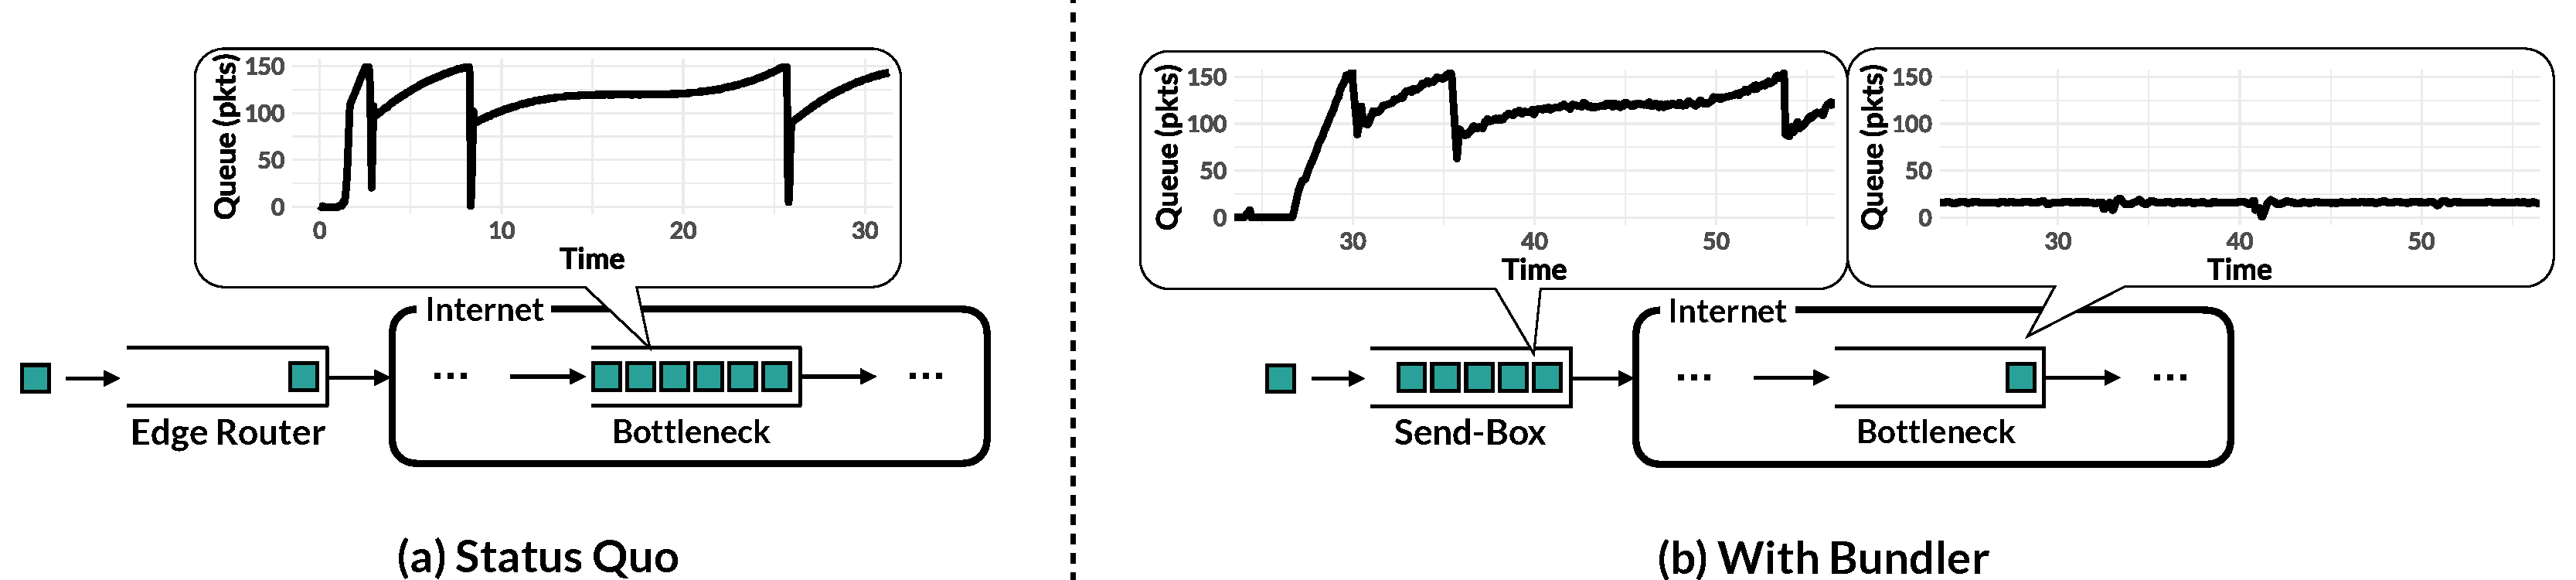
\includegraphics[width=\textwidth]{img/shift-bottleneck-combined}
    \caption{This illustrative example with a single flow shows how \name can take control of queues in the network. The plots show the trend in measured queueing delays at the relevant queue over time. The queue where delays build up can best make scheduling decisions, since it has the most choice between packets to send. Therefore, the \inbox \emph{shifts} the queues to itself to gain scheduling power. }\label{fig:design:shift-bottleneck}
\end{figure*}
%

\an{Is this section too defensive?}
\radhika{also, we need a better title}

Figure~\ref{fig:deploy:arch} provides an example scenario for deploying \name. 
\name aggregates traffic between Domain A and Domain B into the same bundle. 
Then, on egress, the \inbox moves the in-network queues built by the bundled traffic to itself (we describe the specific mechanism in \S\ref{s:design}). 
It can thus enforce desired scheduling policies across the traffic in the bundle.

The performance benefits that this provides are dictated by the following.

\Para{Amount of Aggregation} 
Bundles are naturally \emph{composable}: a subdomain of domain A could deploy its own \name to take control of its fraction of the in-network queues. \an{move to discussion}
%However, the amount of aggregated traffic in a bundle correlates with the scheduling opportunities within it, thus influencing the performance benefits that \name provides. 
\radhika{this is still not the right place to mention composability :)}
However, a traffic bundle, to be useful, must be \emph{heavyweight} enough to drive self-inflicted queueing in the network; these queues, once \name controls them, provide scheduling opportunity.
In our example scenario, the bundle from Domain A to B might be comprised of large amounts of traffic generated by various services (such as email, messaging, video conferencing, video streaming, cloud storage etc.) hosted by the content provider and used by different clients within the enterprise.
We expect many bundles to be heavyweight in practice because a majority of Internet traffic today is owned by a few large content providers who host a wide array of services~\cite{fivecomps, labovitz}. 
Furthermore, it is possible to observe self-inflicted queueing even by sending from a single machine; we take advantage of this in experiments on real Internet paths in \S\ref{s:eval}. \radhika{chop last line?}

\Para{Congestion in the middle of the network} 
Customers already have control over queues that are built within their own domains~\cite{swan, b4, bwe}. \name, therefore, provides benefits when congestion occurs, and queues build up, in the middle of the network (\ie between a \pair).  
So the next question that arises is, does such in-network congestion occur in practice? A recent measurement study~\cite{inferring-interdomain-congestion} indicates that inter-domain links in the network (such as the red bottleneck link in Figure~\ref{fig:deploy:arch}) can indeed experience significant congestion. 
We briefly discuss how the nature of this congestion influences \name's benefits (and provide detailed results in \S\ref{s:eval}). \radhika{make consistent with figure}

\paragraphi{Self-inflicted congestion} This occurs when traffic from a single bundle causes a queue to build up at the bottleneck links in the network, even without any other cross-traffic. It can happen when a small carrier network does not have enough capacity to sustain the large volume of traffic sent by a content provider to a receiving domain, or due to explicit rate limiting commonly done by ISPs~\cite{isp-throttle-1, isp-throttle-2, isp-throttle-3}. In such cases, \name can result in
significant improvements in performance, as it would then have control over the entire queue. In our experiments (\S\ref{s:eval}), we found this to be the case.

\paragraphi{Congestion due to bundled cross-traffic} In-network congestion can further increase in the presence of other cross-traffic (\eg when the peering link between Carrier B and the enterprise in Figure~\ref{fig:deploy:arch} is shared by traffic from multiple sending domains). 
\name continues to provide benefits when the competing flows are part of other bundles from/to other domains because the rate control algorithm at each of the other {\inbox}es would ensure that the in-network queues remain small. Since each \inbox controls its own delays, it can apply the appropriate scheduling policy its the per-bundle queues.
We expect this to become the common form of observed congestion as more domains deploy \name. 

\paragraphi{Congestion due to un-bundled cross-traffic} We now consider the scenario where the cross-traffic includes flows from domains that have not yet deployed a \name. If all such \emph{un-bundled} competing flows are short-lived (up to a few MBs), the bundled traffic still sees significant performance benefits. 
However, if the cross traffic aggressively fills up available buffer space at the bottleneck link, to compete fairly \name would have to push more packets into the network (as described in \S\ref{s:queue-ctl}), relinquishing control over bundled traffic.
This scenario is a limitation of \name's design, since it forces \name to fall back to status-quo performance.
\an{reword} Such flows are unlikely to arrive very frequently~\cite{caida-dataset}. 

\vspace{0.05in}
\paragrapha{Takeaway} While \name must revert to status quo performance in the face of aggressive, buffer-filling cross traffic, in most scenarios it can significantly improve performance.
This, combined with its deployment ease, makes a strong case for deploying \name. 
